% answers.tex —— 2012 年·重庆卷·文科 · 参考答案与详细解析片段
% 由 tools/generate_projects.py 依来源总账自 2012/2012_数学真题_重庆文_试题.md + 2012/2012_数学真题_重庆文_解析正文.md + 2012/2012_数学真题_重庆文_答案要点.md 生成，勿手改（改源 MD 后重跑）

\begin{answer}
\gksolhead{1}{}

\textbf{题目}：

命题“若 $p$ 则 $q$”的逆命题是\mbox{（　　）}

（A）若 $q$ 则 $p$；（B）若 $\neg p$ 则 $\neg q$；（C）若 $\neg q$ 则 $\neg p$；（D）若 $p$ 则 $\neg q$。

\Needspace{4\baselineskip}
\textbf{解析}
“若 $p$ 则 $q$”的逆命题是“若 $q$ 则 $p$”。选 A。

\gkanswer{答案：A。}

\end{answer}
\begin{answer}
\gksolhead{2}{}

\textbf{题目}：

不等式 $\dfrac{x-1}{x+2}<0$ 的解集为\mbox{（　　）}

（A）$(1,+\infty)$；（B）$(-\infty,-2)$；（C）$(-2,1)$；（D）$(-\infty,-2)\cup(1,+\infty)$。

\Needspace{4\baselineskip}
\textbf{解析}
$\dfrac{x-1}{x+2}<0$ 等价于 $(x-1)(x+2)<0$，解得 $-2<x<1$。选 C。

\gkanswer{答案：C。}

\end{answer}
\begin{answer}
\gksolhead{3}{}

\textbf{题目}：

设 $A$，$B$ 为直线 $y=x$ 与圆 $x^2+y^2=1$ 的两个交点，则 $|AB|=$\mbox{（　　）}

（A）$1$；（B）$\sqrt2$；（C）$\sqrt3$；（D）$2$。

\Needspace{4\baselineskip}
\textbf{解析}
\Needspace{5\baselineskip}
由 $y=x$ 与 $x^2+y^2=1$ 得 $2x^2=1$，两交点为 $\left(\dfrac{\sqrt2}2,\dfrac{\sqrt2}2\right)$，$\left(-\dfrac{\sqrt2}2,-\dfrac{\sqrt2}2\right)$，故
\nopagebreak[4]
\[|AB|=\sqrt{(\sqrt2)^2+(\sqrt2)^2}=2.\]
选 D。

\gkanswer{答案：D。}

\end{answer}
\begin{answer}
\gksolhead{4}{}

\textbf{题目}：

$(1-3x)^5$ 的展开式中 $x^3$ 的系数为\mbox{（　　）}

（A）$-270$；（B）$-90$；（C）$90$；（D）$270$。

\Needspace{4\baselineskip}
\textbf{解析}
$x^3$ 项为 $\mathrm C_5^3(-3x)^3=10\times(-27)x^3=-270x^3$。选 A。

\gkanswer{答案：A。}

\end{answer}
\begin{answer}
\gksolhead{5}{}

\textbf{题目}：

$\dfrac{\sin47^\circ-\sin17^\circ\cos30^\circ}{\cos17^\circ}=$\mbox{（　　）}

（A）$-\dfrac{\sqrt3}2$；（B）$-\dfrac12$；（C）$\dfrac12$；（D）$\dfrac{\sqrt3}2$。

\Needspace{4\baselineskip}
\textbf{解析}
\nopagebreak[4]
\[\sin47^\circ=\sin(30^\circ+17^\circ)=\sin30^\circ\cos17^\circ+\cos30^\circ\sin17^\circ,\]
故分子 $=\sin30^\circ\cos17^\circ$，原式 $=\sin30^\circ=\dfrac12$。选 C。

\gkanswer{答案：C。}

\end{answer}
\begin{answer}
\gksolhead{6}{}

\textbf{题目}：

设 $x\in\mathbf R$，向量 $\boldsymbol a=(x,1)$，$\boldsymbol b=(1,-2)$，且 $\boldsymbol a\perp\boldsymbol b$，则 $|\boldsymbol a+\boldsymbol b|=$\mbox{（　　）}

（A）$\sqrt5$；（B）$\sqrt{10}$；（C）$2\sqrt5$；（D）$10$。

\Needspace{4\baselineskip}
\textbf{解析}
\Needspace{5\baselineskip}
由 $\boldsymbol a\perp\boldsymbol b$ 得 $x-2=0$，即 $x=2$。于是 $\boldsymbol a+\boldsymbol b=(3,-1)$，
\nopagebreak[4]
\[|\boldsymbol a+\boldsymbol b|=\sqrt{9+1}=\sqrt{10}.\]
选 B。

\gkanswer{答案：B。}

\end{answer}
\begin{answer}
\gksolhead{7}{}

\textbf{题目}：

已知 $a=\log_23+\log_2\sqrt3$，$b=\log_29-\log_2\sqrt3$，$c=\log_32$，则 $a$，$b$，$c$ 的大小关系是\mbox{（　　）}

（A）$a=b<c$；（B）$a=b>c$；（C）$a<b<c$；（D）$a>b>c$。

\Needspace{4\baselineskip}
\textbf{解析}
\nopagebreak[4]
\[a=\log_2(3\sqrt3),\qquad b=\log_2\frac9{\sqrt3}=\log_2(3\sqrt3),\]
故 $a=b$。又 $a>1$，$c=\log_32<1$，故 $a=b>c$。选 B。

\gkanswer{答案：B。}

\end{answer}
\begin{answer}
\gksolhead{8}{}

\textbf{题目}：

设函数 $f(x)$ 在 $\mathbf R$ 上可导，其导函数为 $f'(x)$，且函数 $f(x)$ 在 $x=-2$ 处取得极小值，则函数 $y=xf'(x)$ 的图象可能是\mbox{（　　）}
\nopagebreak[4]
\begin{center}% 2012 年重庆卷文科第 8 题：y=xf'(x) 的四个图象选项。
% 来源 PDF：普通高考/2012/2012重庆文.pdf，第 1 页（印面 723）第 2 栏。
% 选项 (B) 为零点 x=-2 与 x=0、在 (-2,0) 内为负、两侧为正的图象，即正确答案。
\begin{tikzpicture}[scale=0.78, semithick, >=Stealth, font=\small]
  \foreach \dx/\dy/\lab in {0/0/{(A)}, 5.4/0/{(B)}, 0/-5.2/{(C)}, 5.4/-5.2/{(D)}} {
    \begin{scope}[shift={(\dx,\dy)}]
      \clip (-2.3,-1.9) rectangle (2.3,1.9);
      \draw[->] (-2.4,0) -- (2.4,0) node[right] {$x$};
      \draw[->] (0,-2.0) -- (0,2.0) node[above] {$y$};
      \node[below left] at (0,0) {\scriptsize $O$};
    \end{scope}
    \node[below] at (\dx,\dy-2.35) {\lab};
  }
  % (A)
  \begin{scope}[shift={(0,0)}]
    \clip (-2.3,-1.9) rectangle (2.3,1.9);
    \draw[smooth, domain=-2.3:1.2] plot (\x, {-0.6*\x*(\x+2.4)});
  \end{scope}
  % (B)
  \begin{scope}[shift={(5.4,0)}]
    \clip (-2.3,-1.9) rectangle (2.3,1.9);
    \draw[smooth, domain=-2.3:1.4] plot (\x, {0.55*\x*(\x+2)});
    \node[below] at (-2,-0.05) {\scriptsize $-2$};
  \end{scope}
  % (C)
  \begin{scope}[shift={(0,-5.2)}]
    \clip (-2.3,-1.9) rectangle (2.3,1.9);
    \draw[smooth, domain=-2.3:2.0] plot (\x, {0.8*\x});
  \end{scope}
  % (D)
  \begin{scope}[shift={(5.4,-5.2)}]
    \clip (-2.3,-1.9) rectangle (2.3,1.9);
    \draw[smooth, domain=-2.3:1.4] plot (\x, {-0.55*\x*(\x+2)});
    \node[below] at (-2,-0.05) {\scriptsize $-2$};
  \end{scope}
\end{tikzpicture}
\end{center}
\nopagebreak[4]
\Needspace{4\baselineskip}
\textbf{解析}
$f(x)$ 在 $x=-2$ 处取极小值，故 $x<-2$ 时 $f'(x)<0$，$-2<x$ 时 $f'(x)>0$（在 $-2$ 附近）。

于是 $x<-2$ 时 $xf'(x)>0$；$-2<x<0$ 时 $xf'(x)<0$；$x>0$ 时 $xf'(x)>0$。即图象在 $x=-2$ 与 $x=0$ 处为零，且在 $(-2,0)$ 内为负，在两侧为正。选 B。

\gkanswer{答案：B。}

\end{answer}
\begin{answer}
\gksolhead{9}{}

\textbf{题目}：

设四面体的六条棱的长分别为 $1$，$1$，$1$，$1$，$\sqrt2$ 和 $a$，且长为 $a$ 的棱与长为 $\sqrt2$ 的棱异面，则 $a$ 的取值范围是\mbox{（　　）}

（A）$\left(0,\sqrt2\right)$；（B）$\left(0,\sqrt3\right)$；（C）$\left(1,\sqrt2\right)$；（D）$\left(1,\sqrt3\right)$。

\Needspace{4\baselineskip}
\textbf{解析}
设四面体 $ABCD$ 中 $AB=AC=BD=CD=1$，$BC=\sqrt2$，$AD=a$，则 $a$ 与 $\sqrt2$ 为对棱。

\Needspace{5\baselineskip}
由 $AB^2+AC^2=BC^2$ 知 $\angle BAC=90^\circ$，同理 $\angle BDC=90^\circ$，故 $A$，$D$ 都在以 $BC$ 为直径的球面上，该球半径为 $\dfrac{\sqrt2}2$。于是
\nopagebreak[4]
\[0<AD<2\times\frac{\sqrt2}2=\sqrt2,\]
且 $A$，$D$ 不重合，故 $a\in\left(0,\sqrt2\right)$。选 A。

\gkanswer{答案：A。}

\end{answer}
\begin{answer}
\gksolhead{10}{}

\textbf{题目}：

设函数 $f(x)=x^2-4x+3$，$g(x)=3^x-2$，集合 $M=\{x\in\mathbf R\mid f(g(x))>0\}$，$N=\{x\in\mathbf R\mid g(x)<2\}$，则 $M\cap N$ 为\mbox{（　　）}

（A）$(1,+\infty)$；（B）$(0,1)$；（C）$(-1,1)$；（D）$(-\infty,1)$。

\Needspace{4\baselineskip}
\textbf{解析}
$f(g(x))>0$ 即 $g(x)<1$ 或 $g(x)>3$，也就是 $3^x<3$ 或 $3^x>5$，即 $x<1$ 或 $x>\log_35$。

\Needspace{5\baselineskip}
又 $g(x)<2$ 即 $3^x<4$，$x<\log_34$。因为 $\log_35>\log_34$，故
\nopagebreak[4]
\[M\cap N=(-\infty,1).\]
选 D。

\gkanswer{答案：D。}

\end{answer}
\begin{answer}
\gksolhead{11}{}

\textbf{题目}：

首项为 $1$，公比为 $2$ 的等比数列的前 $4$ 项和 $S_4=$\gkblank{}。

\Needspace{4\baselineskip}
\textbf{解析}
\nopagebreak[4]
\[S_4=\frac{1(1-2^4)}{1-2}=15.\]

\gkanswer{答案：$15$。}

\end{answer}
\begin{answer}
\gksolhead{12}{}

\textbf{题目}：

若 $f(x)=(x+a)(x-4)$ 为偶函数，则实数 $a=$\gkblank{}。

\Needspace{4\baselineskip}
\textbf{解析}
$f(x)=x^2+(a-4)x-4a$。若为偶函数，则一次项系数 $a-4=0$，故 $a=4$。

\gkanswer{答案：$4$。}

\end{answer}
\begin{answer}
\gksolhead{13}{}

\textbf{题目}：

设 $\triangle ABC$ 的内角 $A$，$B$，$C$ 的对边分别为 $a$，$b$，$c$，且 $a=1$，$b=2$，$\cos C=\dfrac14$，则 $\sin B=$\gkblank{}。

\Needspace{4\baselineskip}
\textbf{解析}
\Needspace{5\baselineskip}
由余弦定理 $c^2=a^2+b^2-2ab\cos C=1+4-4\times\dfrac14=4$，故 $c=2$。又
\nopagebreak[4]
\[\sin C=\sqrt{1-\frac1{16}}=\frac{\sqrt{15}}4,\]
\Needspace{5\baselineskip}
由正弦定理
\nopagebreak[4]
\[\sin B=\frac{b\sin C}c=\frac{2\times\frac{\sqrt{15}}4}2=\frac{\sqrt{15}}4.\]

\gkanswer{答案：$\dfrac{\sqrt{15}}4$。}

\end{answer}
\begin{answer}
\gksolhead{14}{}

\textbf{题目}：

设 $P$ 为直线 $y=\dfrac b{3a}x$ 与双曲线 $\dfrac{x^2}{a^2}-\dfrac{y^2}{b^2}=1$（$a>0$，$b>0$）左支的交点，$F_1$ 是左焦点，$PF_1$ 垂直于 $x$ 轴，则双曲线的离心率 $e=$\gkblank{}。

\Needspace{4\baselineskip}
\textbf{解析}
\Needspace{5\baselineskip}
$PF_1\perp x$ 轴，故 $P\left(-c,\dfrac{bc}{3a}\right)$（左支）。又 $P$ 在双曲线上，$x=-c$ 时
\nopagebreak[4]
\[\frac{c^2}{a^2}-\frac{y^2}{b^2}=1\ \Rightarrow\ |y|=\frac{b^2}a.\]
\Needspace{5\baselineskip}
故 $\dfrac{bc}{3a}=\dfrac{b^2}a$，即 $c=3b$。由 $c^2=a^2+b^2$ 得 $a^2=8b^2$，于是
\nopagebreak[4]
\[e=\frac ca=\frac{3b}{2\sqrt2b}=\frac{3\sqrt2}4.\]

\gkanswer{答案：$\dfrac{3\sqrt2}4$。}

\end{answer}
\begin{answer}
\gksolhead{15}{}

\textbf{题目}：

某艺校在一天的 $6$ 节课中随机安排语文、数学、外语三门文化课和其他三门艺术课各 $1$ 节，则在课表上的相邻两节文化课之间至少间隔 $1$ 节艺术课的概率为\gkblank{}。（用数字作答）

\Needspace{4\baselineskip}
\textbf{解析}
\Needspace{5\baselineskip}
三门文化课两两不相邻的排法：先排三门艺术课（$3!$ 种），形成 $4$ 个空位，选 $3$ 个放文化课（$\mathrm C_4^3$ 种，$3!$ 种排列），共
\nopagebreak[4]
\[3!\times\mathrm C_4^3\times3!=144\]
\Needspace{5\baselineskip}
种。总排法 $6!=720$ 种，故概率为
\nopagebreak[4]
\[\frac{144}{720}=\frac15.\]

\gkanswer{答案：$\dfrac15$。}

\end{answer}
\begin{answer}
\gksolhead{16}{}

\textbf{题目}：

已知 $\{a_n\}$ 为等差数列，且 $a_1+a_3=8$，$a_2+a_4=12$。

（1） 求 $\{a_n\}$ 的通项公式；

（2） 记 $\{a_n\}$ 的前 $n$ 项和为 $S_n$，若 $a_1$，$a_k$，$a_{k+2}$ 成等比数列，求正整数 $k$ 的值。

\Needspace{4\baselineskip}
\textbf{解析}
\Needspace{5\baselineskip}
\textbf{（1）} 设公差为 $d$，则
\nopagebreak[4]
\[a_1+a_3=2a_1+2d=8,\qquad a_2+a_4=2a_1+4d=12,\]
\Needspace{5\baselineskip}
解得 $d=2$，$a_1=2$，故
\nopagebreak[4]
\[a_n=2n.\]

\Needspace{5\baselineskip}
\textbf{（2）} $a_1=2$，$a_k=2k$，$a_{k+2}=2k+4$。由等比得
\nopagebreak[4]
\[(2k)^2=2(2k+4),\]
即 $k^2-k-2=0$，解得 $k=2$（$k$ 为正整数）。

\gkanswer{答案（1）：$a_n=2n$。}

\gkanswer{答案（2）：$k=2$。}

\end{answer}
\begin{answer}
\gksolhead{17}{}

\textbf{题目}：

已知函数 $f(x)=ax^3+bx+c$ 在点 $x=2$ 处取得极值 $c-16$。

（1） 求 $a$，$b$ 的值；

（2） 若 $f(x)$ 有极大值 $28$，求 $f(x)$ 在 $[-3,3]$ 上的最小值。

\Needspace{4\baselineskip}
\textbf{解析}
\Needspace{5\baselineskip}
\textbf{（1）} $f'(x)=3ax^2+b$。由 $x=2$ 处取极值 $c-16$ 得
\nopagebreak[4]
\[f'(2)=12a+b=0,\qquad f(2)=8a+2b+c=c-16,\]
\Needspace{5\baselineskip}
即 $12a+b=0$，$4a+b=-8$。相减得 $8a=8$，故
\nopagebreak[4]
\[a=1,\qquad b=-12.\]

\Needspace{5\baselineskip}
\textbf{（2）} $f(x)=x^3-12x+c$，$f'(x)=3x^2-12$，驻点 $x=\pm2$。$x=-2$ 为极大值点：
\nopagebreak[4]
\[f(-2)=-8+24+c=16+c=28,\]
故 $c=12$，$f(x)=x^3-12x+12$。

在 $[-3,3]$ 上比较：$f(-3)=21$，$f(-2)=28$，$f(2)=-4+12=8$，$f(3)=27-36+12=3$。故最小值为 $3$（在 $x=3$ 处）。

\gkanswer{答案（1）：$a=1$，$b=-12$。}

\gkanswer{答案（2）：$3$。}

\end{answer}
\begin{answer}
\gksolhead{18}{}

\textbf{题目}：

甲、乙两人轮流投篮，每人每次投一球。约定甲先投且先投中者获胜，一直到有人获胜或每人都已投球 $3$ 次时投篮结束。设甲每次投篮投中的概率为 $\dfrac13$，乙每次投篮投中的概率为 $\dfrac12$，且各次投篮互不影响。

（1） 求乙获胜的概率；

（2） 求投篮结束时乙只投了 $2$ 个球的概率。

\Needspace{4\baselineskip}
\textbf{解析}
记甲投中概率 $\dfrac13$，乙投中概率 $\dfrac12$。

\Needspace{5\baselineskip}
\textbf{（1）} 乙获胜需甲未中且乙中：
\nopagebreak[4]
\[P=\frac23\cdot\frac12+\frac23\cdot\frac12\cdot\frac23\cdot\frac12+\left(\frac23\cdot\frac12\right)^3=\frac13+\frac19+\frac1{27}=\frac{13}{27}.\]

\textbf{（2）} 乙只投 $2$ 个球的情形：
乙第 $2$ 球投中而获胜：$\left(\dfrac23\cdot\dfrac12\right)^2=\dfrac19$；
或甲第 $3$ 球投中而获胜（此前两轮双方均未中）：$\left(\dfrac23\cdot\dfrac12\right)^2\cdot\dfrac13=\dfrac1{27}$。

\Needspace{5\baselineskip}
故
\nopagebreak[4]
\[P=\frac19+\frac1{27}=\frac4{27}.\]

\gkanswer{答案（1）：$\dfrac{13}{27}$。}

\gkanswer{答案（2）：$\dfrac4{27}$。}

\end{answer}
\begin{answer}
\gksolhead{19}{}

\textbf{题目}：

设函数 $f(x)=A\sin(\omega x+\varphi)$（其中 $A>0$，$\omega>0$，$-\pi<\varphi\leqslant\pi$）在 $x=\dfrac\pi6$ 处取得最大值 $2$，其图象与 $x$ 轴的相邻两个交点的距离为 $\dfrac\pi2$。

（1） 求 $f(x)$ 的解析式；

（2） 求函数 $g(x)=\dfrac{6\cos^4x-\sin^2x-1}{f\left(x+\dfrac\pi6\right)}$ 的值域。

\Needspace{4\baselineskip}
\textbf{解析}
\Needspace{5\baselineskip}
\textbf{（1）} 最大值为 $2$，故 $A=2$；相邻零点距离为 $\dfrac T2=\dfrac\pi2$，故 $T=\pi$，$\omega=2$。由 $x=\dfrac\pi6$ 处取最大值：
\nopagebreak[4]
\[2\cdot\frac\pi6+\varphi=\frac\pi2,\]
\Needspace{5\baselineskip}
得 $\varphi=\dfrac\pi6$，故
\nopagebreak[4]
\[f(x)=2\sin\left(2x+\frac\pi6\right).\]

\Needspace{5\baselineskip}
\textbf{（2）}
\nopagebreak[4]
\[f\left(x+\frac\pi6\right)=2\sin\left(2x+\frac\pi2\right)=2\cos2x.\]
\Needspace{5\baselineskip}
分子：
\nopagebreak[4]
\[6\cos^4x-\sin^2x-1=6\cos^4x+\cos^2x-2=(3\cos^2x+2)(2\cos^2x-1).\]
\Needspace{5\baselineskip}
故
\nopagebreak[4]
\[g(x)=\frac{(3\cos^2x+2)(2\cos^2x-1)}{2\cos2x}=\frac{3\cos^2x+2}2=\frac{7+3\cos2x}4.\]
\Needspace{5\baselineskip}
由 $\cos2x\in[-1,1]$ 且 $\cos2x\neq0$，得值域
\nopagebreak[4]
\[\left[1,\frac74\right)\cup\left(\frac74,\frac52\right].\]

\gkanswer{答案（1）：$f(x)=2\sin\left(2x+\dfrac\pi6\right)$。}

\gkanswer{答案（2）：$\left[1,\dfrac74\right)\cup\left(\dfrac74,\dfrac52\right]$。}

\end{answer}
\begin{answer}
\gksolhead{20}{}

\textbf{题目}：

如图，在直三棱柱 $ABC-A_1B_1C_1$ 中，$AB=4$，$AC=BC=3$，$D$ 为 $AB$ 的中点。

（1） 求异面直线 $CC_1$ 和 $AB$ 的距离；

（2） 若 $AB_1\perp A_1C$，求二面角 $A_1-CD-B_1$ 的平面角的余弦值。
\nopagebreak[4]
\begin{center}% 2012 年重庆卷文科第 20 题：直三棱柱 ABC-A1B1C1，D 为 AB 中点。
% 来源 PDF：普通高考/2012/2012重庆文.pdf，第 2 页（印面 724）第 2 栏。
% 投影：screen(x,y,z) = (x + 0.45y, 0.55y + 0.75z)，取 AB=4、CD=√5、高 2√2。
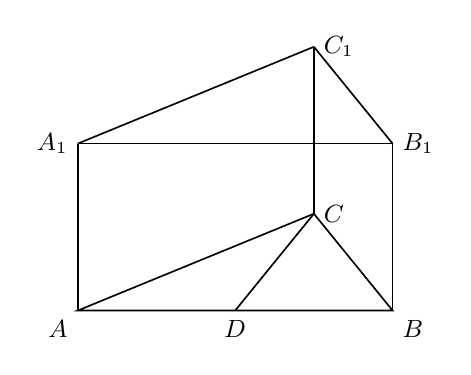
\begin{tikzpicture}[semithick, font=\small]
  \coordinate (A)  at (-2,0);
  \coordinate (B)  at (2,0);
  \coordinate (C)  at (1.0,1.23);
  \coordinate (D)  at (0,0);
  \coordinate (A1) at (-2,2.12);
  \coordinate (B1) at (2,2.12);
  \coordinate (C1) at (1.0,3.35);
  \draw (A) -- (B) -- (C) -- cycle;
  \draw (A) -- (A1);
  \draw (B) -- (B1);
  \draw (C) -- (C1);
  \draw (A1) -- (B1);
  \draw (B1) -- (C1);
  \draw (A1) -- (C1);
  \draw (C) -- (D);
  \node[below left] at (A) {$A$};
  \node[below right] at (B) {$B$};
  \node[right] at (C) {$C$};
  \node[below] at (D) {$D$};
  \node[left] at (A1) {$A_1$};
  \node[right] at (B1) {$B_1$};
  \node[right] at (C1) {$C_1$};
\end{tikzpicture}
\end{center}
\nopagebreak[4]
\Needspace{4\baselineskip}
\textbf{解析}
\Needspace{5\baselineskip}
\textbf{（1）} 直三棱柱中 $CC_1\perp$ 平面 $ABC$，故 $CC_1$ 与 $AB$ 的距离等于 $C$ 到 $AB$ 的距离。$\triangle ABC$ 中 $AC=BC=3$，$AB=4$，$D$ 为 $AB$ 中点，故
\nopagebreak[4]
\[CD=\sqrt{3^2-2^2}=\sqrt5.\]

\Needspace{5\baselineskip}
\textbf{（2）} 取 $D$ 为原点，$AB$ 为 $x$ 轴，$DC$ 为 $y$ 轴，$DD_1$ 为 $z$ 轴：
\nopagebreak[4]
\[A(-2,0,0),\ B(2,0,0),\ C(0,\sqrt5,0),\ A_1(-2,0,h),\ B_1(2,0,h).\]
\Needspace{5\baselineskip}
由 $AB_1\perp A_1C$：
\nopagebreak[4]
\[\overrightarrow{AB_1}\cdot\overrightarrow{A_1C}=(4,0,h)\cdot(2,\sqrt5,-h)=8-h^2=0,\]
故 $h=2\sqrt2$。

\Needspace{5\baselineskip}
平面 $A_1CD$ 的法向量
\nopagebreak[4]
\[\boldsymbol n_1=\overrightarrow{DC}\times\overrightarrow{DA_1}=(0,\sqrt5,0)\times(-2,0,2\sqrt2)=(2\sqrt{10},0,2\sqrt5),\]
\Needspace{5\baselineskip}
平面 $B_1CD$ 的法向量
\nopagebreak[4]
\[\boldsymbol n_2=\overrightarrow{DC}\times\overrightarrow{DB_1}=(2\sqrt{10},0,-2\sqrt5).\]
\Needspace{5\baselineskip}
设二面角为 $\theta$，则
\nopagebreak[4]
\[\cos\theta=\frac{\boldsymbol n_1\cdot\boldsymbol n_2}{|\boldsymbol n_1||\boldsymbol n_2|}=\frac{40-20}{60}=\frac13.\]
故所求余弦值为 $\dfrac13$。

\gkanswer{答案（1）：$\sqrt5$。}

\gkanswer{答案（2）：$\dfrac13$。}

\end{answer}
\begin{answer}
\gksolhead{21}{}

\textbf{题目}：

如图，设椭圆的中心为原点 $O$，长轴在 $x$ 轴上，上顶点为 $A$，左、右焦点分别为 $F_1$，$F_2$，线段 $OF_1$，$OF_2$ 的中点分别为 $B_1$，$B_2$，且 $\triangle AB_1B_2$ 是面积为 $4$ 的直角三角形。

（1） 求该椭圆的离心率和标准方程；

（2） 过 $B_1$ 作直线交椭圆于 $P$，$Q$ 两点，使 $PB_2\perp QB_2$，求 $\triangle PB_2Q$ 的面积。
\nopagebreak[4]
\begin{center}% 2012 年重庆卷文科第 21 题：椭圆上顶点 A、焦点 F1、F2 与 OF 中点 B1、B2。
% 来源 PDF：普通高考/2012/2012重庆文.pdf，第 2 页（印面 724）第 3 栏。
% 按 (1) 的结果 a=2√5、b=2、c=4 作图：A(0,2)，B1(-2,0)，B2(2,0)。
\begin{tikzpicture}[scale=0.62, semithick, >=Stealth, font=\small]
  \draw (0,0) ellipse (4.472 and 2);
  \draw[->] (-5.6,0) -- (5.8,0) node[right] {$x$};
  \draw[->] (0,-3.0) -- (0,3.2) node[above] {$y$};
  \coordinate (A) at (0,2);
  \coordinate (F1) at (-4,0);
  \coordinate (F2) at (4,0);
  \coordinate (B1) at (-2,0);
  \coordinate (B2) at (2,0);
  \fill (A) circle (2.4pt);
  \fill (F1) circle (2.4pt);
  \fill (F2) circle (2.4pt);
  \fill (B1) circle (2.4pt);
  \fill (B2) circle (2.4pt);
  \node[above] at (A) {$A$};
  \node[below left] at (F1) {$F_1$};
  \node[below right] at (F2) {$F_2$};
  \node[below left] at (B1) {$B_1$};
  \node[below right] at (B2) {$B_2$};
  \node[below left] at (0,0) {$O$};
  \draw (A) -- (B1) -- (B2) -- cycle;
\end{tikzpicture}
\end{center}
\nopagebreak[4]
\Needspace{4\baselineskip}
\textbf{解析}
\Needspace{5\baselineskip}
\textbf{（1）} 设椭圆 $\dfrac{x^2}{a^2}+\dfrac{y^2}{b^2}=1$，$A(0,b)$，$B_1\left(-\dfrac c2,0\right)$，$B_2\left(\dfrac c2,0\right)$。$\triangle AB_1B_2$ 为等腰三角形，直角必在 $A$ 处，故
\nopagebreak[4]
\[\overrightarrow{AB_1}\cdot\overrightarrow{AB_2}=\left(-\frac c2,-b\right)\cdot\left(\frac c2,-b\right)=-\frac{c^2}4+b^2=0,\]
\Needspace{5\baselineskip}
即 $b=\dfrac c2$。又面积
\nopagebreak[4]
\[S=\frac12\cdot c\cdot b=\frac12\cdot c\cdot\frac c2=4,\]
\Needspace{5\baselineskip}
得 $c=4$，$b=2$，$a^2=b^2+c^2=20$。故
\nopagebreak[4]
\[e=\frac ca=\frac4{2\sqrt5}=\frac{2\sqrt5}5,\qquad \frac{x^2}{20}+\frac{y^2}4=1.\]

\Needspace{5\baselineskip}
\textbf{（2）} $B_1(-2,0)$，$B_2(2,0)$。设过 $B_1$ 的直线 $y=k(x+2)$，代入椭圆得
\nopagebreak[4]
\[(1+5k^2)x^2+20k^2x+20k^2-20=0.\]
\Needspace{5\baselineskip}
设 $P(x_1,y_1)$，$Q(x_2,y_2)$，则
\nopagebreak[4]
\[x_1+x_2=-\frac{20k^2}{1+5k^2},\qquad x_1x_2=\frac{20k^2-20}{1+5k^2}.\]
\Needspace{5\baselineskip}
由 $PB_2\perp QB_2$：
\nopagebreak[4]
\[(x_1-2)(x_2-2)+y_1y_2=0,\]
\Needspace{5\baselineskip}
即
\nopagebreak[4]
\[(1+k^2)x_1x_2+(2k^2-2)(x_1+x_2)+4(1+k^2)=0.\]
代入并化简得 $64k^2-16=0$，故 $k^2=\dfrac14$。

\Needspace{5\baselineskip}
此时 $|x_1-x_2|=\dfrac{16\sqrt{10}}9$。$\triangle PB_2Q$ 的面积为
\nopagebreak[4]
\[S=\frac12|PQ|\cdot d(B_2,l)=\frac12\sqrt{1+k^2}|x_1-x_2|\cdot\frac{4|k|}{\sqrt{1+k^2}}=2|k||x_1-x_2|=\frac{16\sqrt{10}}9.\]

\gkanswer{答案（1）：$e=\dfrac{2\sqrt5}5$，$\dfrac{x^2}{20}+\dfrac{y^2}4=1$。}

\gkanswer{答案（2）：$\dfrac{16\sqrt{10}}9$。}

\end{answer}